\documentclass[a4paper,11pt,fleqn]{report}

\usepackage{acronym}
\usepackage{amsmath,amssymb,amsfonts}
\usepackage{booktabs}
\usepackage[dvipsnames]{xcolor}
\usepackage[margin=30mm]{geometry}
\usepackage{graphicx}
%	\graphicspath{
%		{.../Graphics/}
%	}
\graphicspath{{graphics/}}
\usepackage{hyperref}
	\hypersetup{
		colorlinks=true,
		linkcolor=blue,
		filecolor=blue,
		urlcolor=blue,
		citecolor=blue
	}
\usepackage[sort&compress]{natbib}
	\bibliographystyle{apalike}
\usepackage[mark]{gitinfo2}
 \renewcommand{\gitMark}{Branch:\,\gitBranch\,@\,\gitAbbrevHash{}; Author:\,\gitAuthorName; Date:\,\gitAuthorIsoDate~\textbullet{}}
\usepackage{url}

\begin{document}
%===============================================================
% Frontmatter and title page to be added manually at the end
%===============================================================
\thispagestyle{empty}
\begin{center}
{\huge \textit{`e-casa'} - Eco-friendly Household Waste System\\Part II}
\vspace{20mm} \\
{\Large Group 6}
\vfill

A project report in partial fulfilment of the requirements for the subject\\
\vspace{10mm}
{\Large \textsc{Systems Engineering (BSS 410)}} \\
\vfill
%
in the \\
\vspace{20mm}
%
{\Large \textsc{Faculty of Engineering, Built Environment, and \\ 
Information Technology}}\\
%
\vspace{10mm}
{\Large\textsc{University of Pretoria}} \\
%
\vfill
%
\today
\end{center}

\textit{`e-casa'} - Eco-friendly Household Waste System
\pagenumbering{roman}

\chapter*{Executive Summary}
The aim of this project is to create a System of Systems (SoS), that will not only reduce the waste produced by a generic household but do so by increasing value to the user. The final deliverable for this project will be a report that details the needs analysis, conceptual design, feasibility and risk assessment for the SoS. The coneptual design of this SoS will be done with the use of \textit{Core 9 Software} to capture all identified needs accurately and produce system design documentation.

\tableofcontents
\listoffigures\addcontentsline{toc}{chapter}{List of Figures}
\listoftables\addcontentsline{toc}{chapter}{List of Tables}

\chapter*{Acronyms}
\addcontentsline{toc}{chapter}{Acronyms}
\begin{acronym}[ABCDEF]
\acro{e-casa}{Eco-friendly Household Waste System}
\acro{SD}{System Dynamics}
\end{acronym}

\chapter{Introduction and Background}
\pagenumbering{arabic}
\setcounter{page}{1}
\acresetall

\section{Problem Background} \label{sec: Problem Background}
 Households consume and produce a variety of products and wastes. Products may take the form of food items, municipal water, electricity and other consumables which are used and then discarded, exiting the household as waste. For example, food clippings from preparing dinner or paper-based packaging is often discarded into dustbins alongside plastic waste to be collected and transported elsewhere. Water used at bathroom sinks is disposed of and sent into the municipal water system. Each type of waste generated by a typical residential household requires proceeding systems that will either store, repurpose or discard the waste.
  
Recent trends have made the consumer market ecologically aware of their own waste generation and many systems have been created to reduce the total waste output of a household. Such products include grey water systems, recycling bins and compost containers. There is a growing need for these systems but presently no solution on the market that integrates all systems into one comprehensive system for homeowners to make use of.
  
Because these systems operate independently, the outputs of one system are often not used as inputs to another. Integrating these systems to operate together could provide more value to the user and further reduce household waste. For e.g. using food clippings to create a compost heap and grow plants and foods in one's garden instead of disposing food clippings in a general waste bin and purchasing compost from a store.

\section{Project Objective} \label{sec: Project Objective}

\chapter{Concept Development Stage}
\section{Needs Analysis Phase} \label{sec: Needs Analysis Phase}
\subsection{Operational Need} \label{Ssec: Operational Need}
\textcolor{red}{\textbf{Operational Need} - The name of the system to be developed and a descriptive representation of the problem to be addressed using letters, figures, charts, photos etc as deemed necessary. Is it a new system from the scratch? Is it a major upgrade of an existing system? Any market opportunities/technological capability in terms of availability and cost? Etc.}

\ac{e-casa} is a sunstainable household waste management system intended to fulfuill the increasingly prevalent need for sustainable living. The need for individuals and households to consume and dispose of resources in a more sustainable manner is becoming ever more pertinent because of increasing strain on the world's most essential natural resources such as water and coal. The need is driven by the requirement for individuals (and society as a whole) to reduce their negative impact on the environment by re-use, recycling and minimising resource use as these natural resources become more scarce. Successfully meeting this need will not only improve living conditions for societies but importantly alleviate pressure on governments and municipalities who have to manage and supply these resources.
Although regulation does not yet fully drive this need, government encourages and sometimes imposes restrictions to ensure responsible water and fuel source use. This is important to develop a sustainable mindset and awareness of waste generation. Because regulation is still limited on use of these resources the onus lies with society and individuals who are aware of and want to mitigate their negative impact on the environment.

\ac{e-casa} is aimed at fulfilling the operational need of sustainable living for households by providing a system that makes it possible to manage and dispose of waste responsibly while simultaneously minimising water consumption. \ac{e-casa} is also expected to provide long-term financial benefits to the user in the form of reduced water consumption costs and grocery bills (with some homegrown foods). Furthermore, there is the expected intangible benefit of the system of knowing one's adverse impact on the environment is mitigated.

Due to a lack of solutions currently on the market, there is an opportunity to enter a gap in the market with \ac{e-casa}. However, this gap is anticipated to be small in size as this product will mainly be aimed at high income individuals aware of (and wanting to reduce) their impact on the environment. There is also an opportunity to market this system as a product to middle class individuals who have sufficient capital to purchase such a system now in order to reap the aforementioned financial savings down the line. However, this extension will likely only be beneficial if the financial savings are substantial enough to persuade these customers.\\

\subsection{Operational Objectives}
\textcolor{red}{\textbf{Requirements Analysis} - what exactly do you want to do in this problem space? Which component(s) of the operational need will you be addressing?}\\

The overarching objective that \ac{e-casa} is intended to fulfil is to provide sustainable household waste management. This objective is deconstructed into three primary objectives, namely: \textit{Provide Waste Storage}, \textit{Reduce Water Consumption} and \textit{Provide long-term cost savings}. Figure~\ref{fig: ecasaOT} shows the operational objectives of the \ac{e-casa} system.\\

\textcolor{red}{*We need an objective tree of our own here that resembles Figure~\ref{fig: ObjectiveTreeStructure}. Figure~\ref{fig: ecasaOT} is a work in progress of that so far.}

\begin{figure}[h!]
\begin{center}
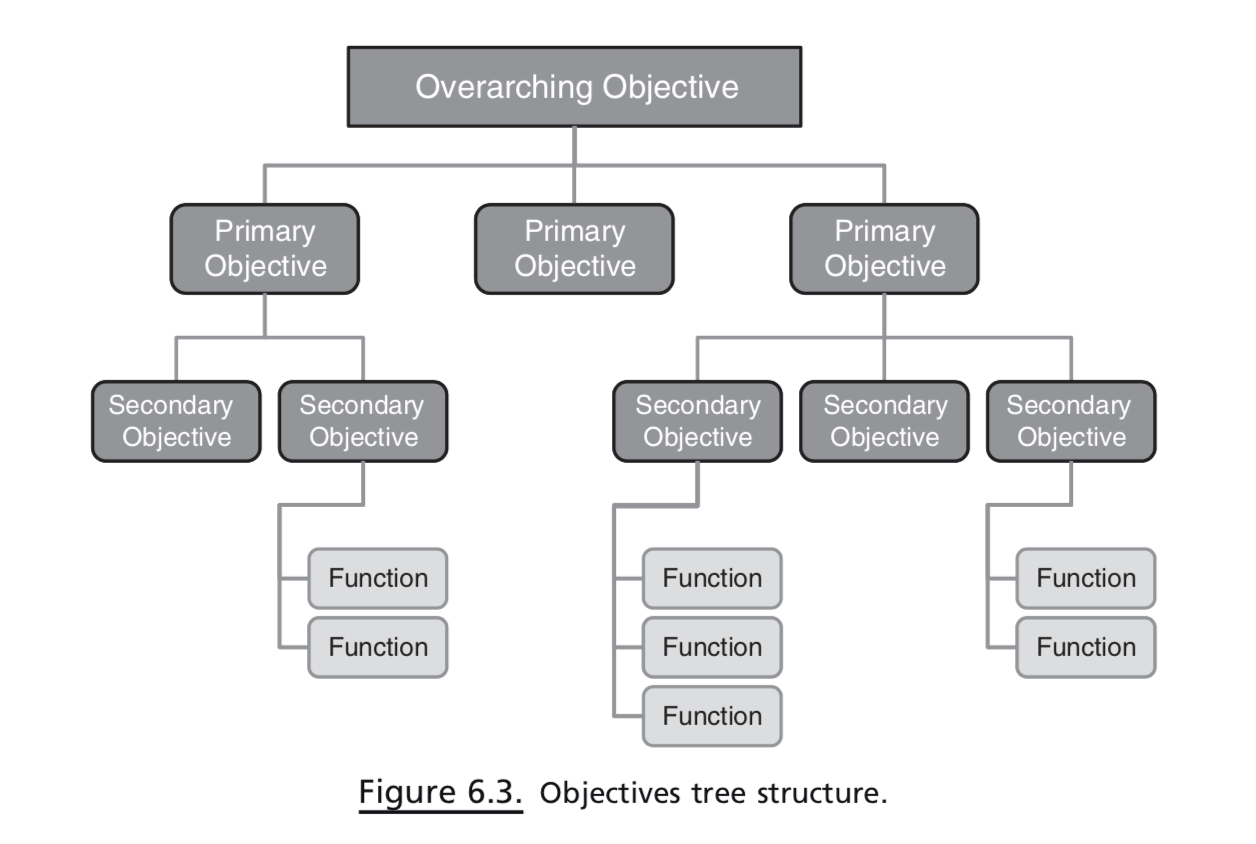
\includegraphics[scale = 0.6]{Objective_Tree_Structure.png}
\caption{Objective Tree Structure}
\label{fig: ObjectiveTreeStructure}
\end{center}
\end{figure}

\begin{figure}[h!]
\begin{center}
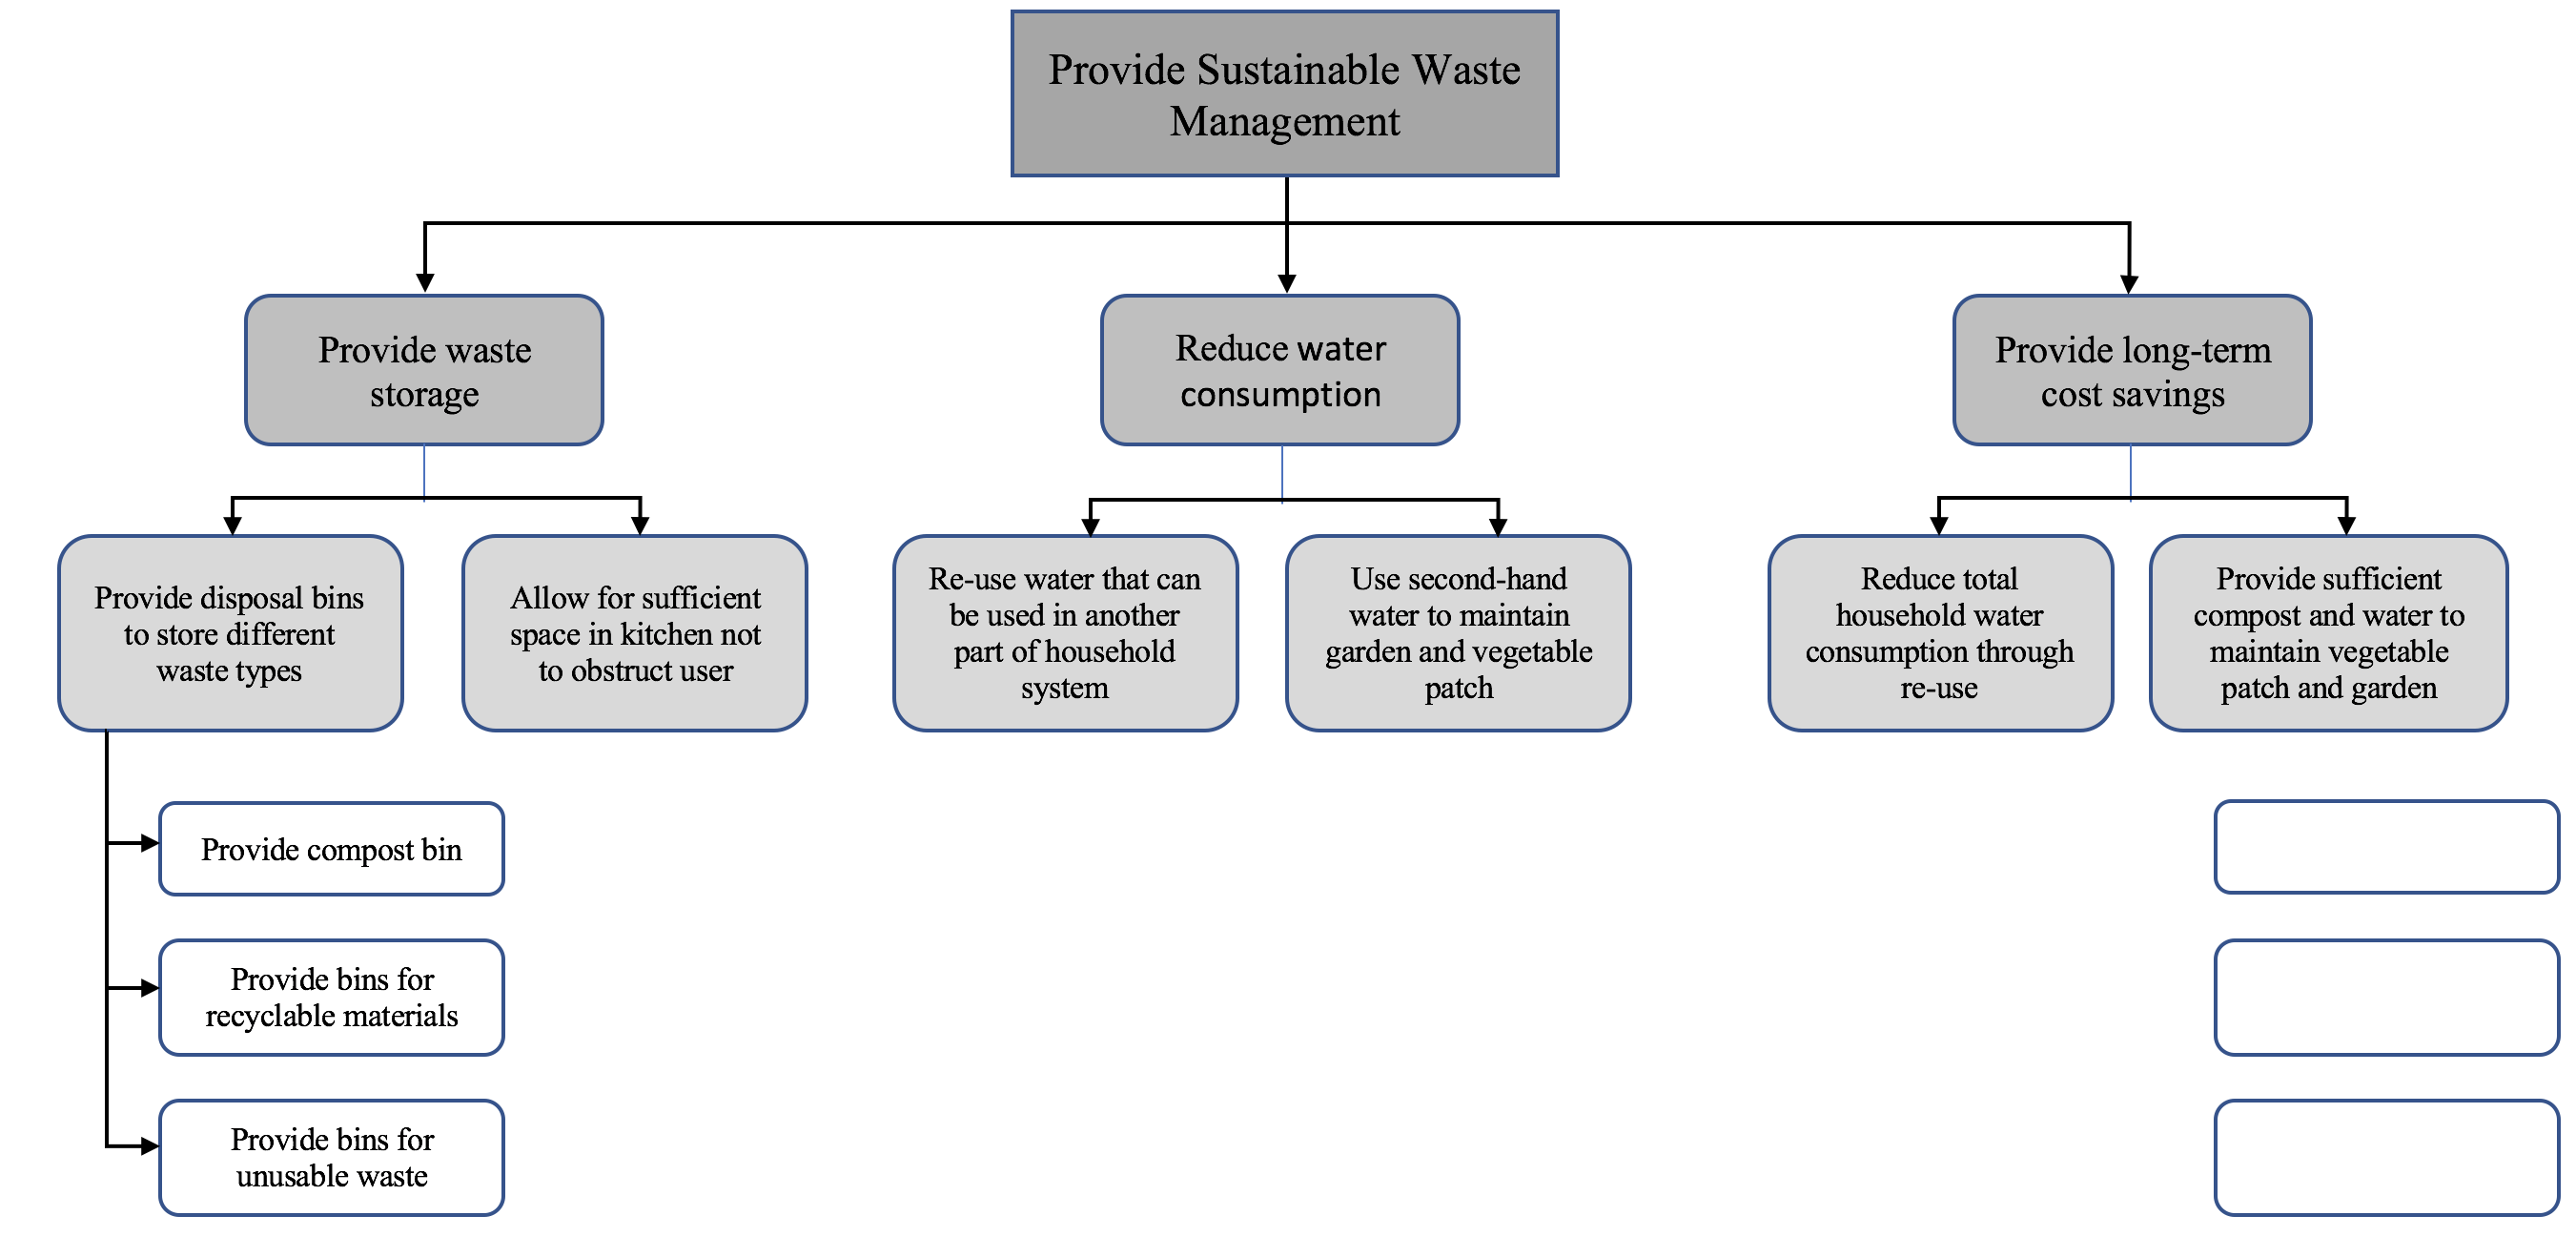
\includegraphics[scale = 0.34]{ecasa_OT.png}
\caption{e-casa Objective Tree Structure}
\label{fig: ecasaOT}
\end{center}
\end{figure}

\subsection{Functional Definition}
\textcolor{red}{What initial functions/processes/capabilities need to come on board to
achieve the stated objectives?}\\

\noindent\textbf{Provide Waste Storage} - Sort waste according to its composition: paper, plastic, glass, organic material, e-waste and unusable waste. Organic material will then be retained within the household for composting and other waste types removed from the household system for the local municipality waste collection service to pick up.\\

\noindent\textbf{Reduce Water Consumption} - A water re-use funciton must be provided to discern which water must be retained by the hosehold for use and which must be discarded into the municipal system based on the origin of the water. ie. Waste water from the toilet must be discarded into the municipal system but used water from the bathroom sink must be retained for re-use to flush the toilet or water the household vegetable patch. This function will also add value to the local municipality by reduce waste output and the volume of water that must be processed.\\

\noindent\textbf{Provide Long-term Cost Savings} - Effective utilisation (re-use) of water and organic waste will reduce the amount of water that needs to be purchased from the municipality, compost that needs to be purchased and eventually groceries that need to be bought. This functionality is essential to reduce the input costs to the household system and provide value to the system user.

\subsection{Feasibility Definition}
Physical Definition - Visualisation of the physical elements/hardware/software/technology
etc. 

gareth was here

\subsection{Need Validation}
\textbf{Design Validation}

\section{Concept Exploration}
\subsection{Operational Requirements Analysis}
analysing the stated operational requirements in terms of their
objectives. Restating, redefining or amplifying (as required) to provide
specificity, independence and consistency among different
objectives

\subsection{Performance Requirements Formulation}
Translating operational requirements into subsystem functions and defining a necessary and sufficient set of performance characteristics reflecting the functions essential to meeting the system’s operational requirements. Formulating the performance parameters required to meet the stated operational requirements.

\subsection{Implementation of Concept Exploration}
Exploring a range of feasible implementation technologies and concepts offering a variety of potentially advantageous options 

\subsection{Performance Requirements Validation}
Conducting effectiveness analyses to define a set of performance requirements that accommodate the full range of desirable system concepts and validating the conformity of these requirements with the stated operational objectives and refining the requirements if necessary. 

\section{Concept Definition}
\subsection{Performance Requirement Analysis}
Analysing the system performance requirements and relate them with operational objectives refining the requirements as necessary to include unstated constraints and quantifying qualitative requirements where possible. 

\subsection{Functional Analysis and Formulation} 
Allocating subsystem functions to the component level in terms of system functional elements and defining element interactions, developing functional architectural products, and formulating preliminary functional requirements corresponding to the assigned functions. 

\subsection{Concept Selection}
Synthesizing alternative technological approaches and component configurations designed to performance requirements; developing physical architectural products; and conducting trade-off studies among performance, risk, cost, and schedule to select the preferred system concept, defined in terms of components and architectures. 

\subsection{Concept Validation}
Conducting system analyses and simulations to confirm that the selected concept meets requirements and is superior to its competitors and refining the concept as may be necessary. 

\chapter{Engineering Development Phase}


\begin{figure}[h!]
\begin{center}
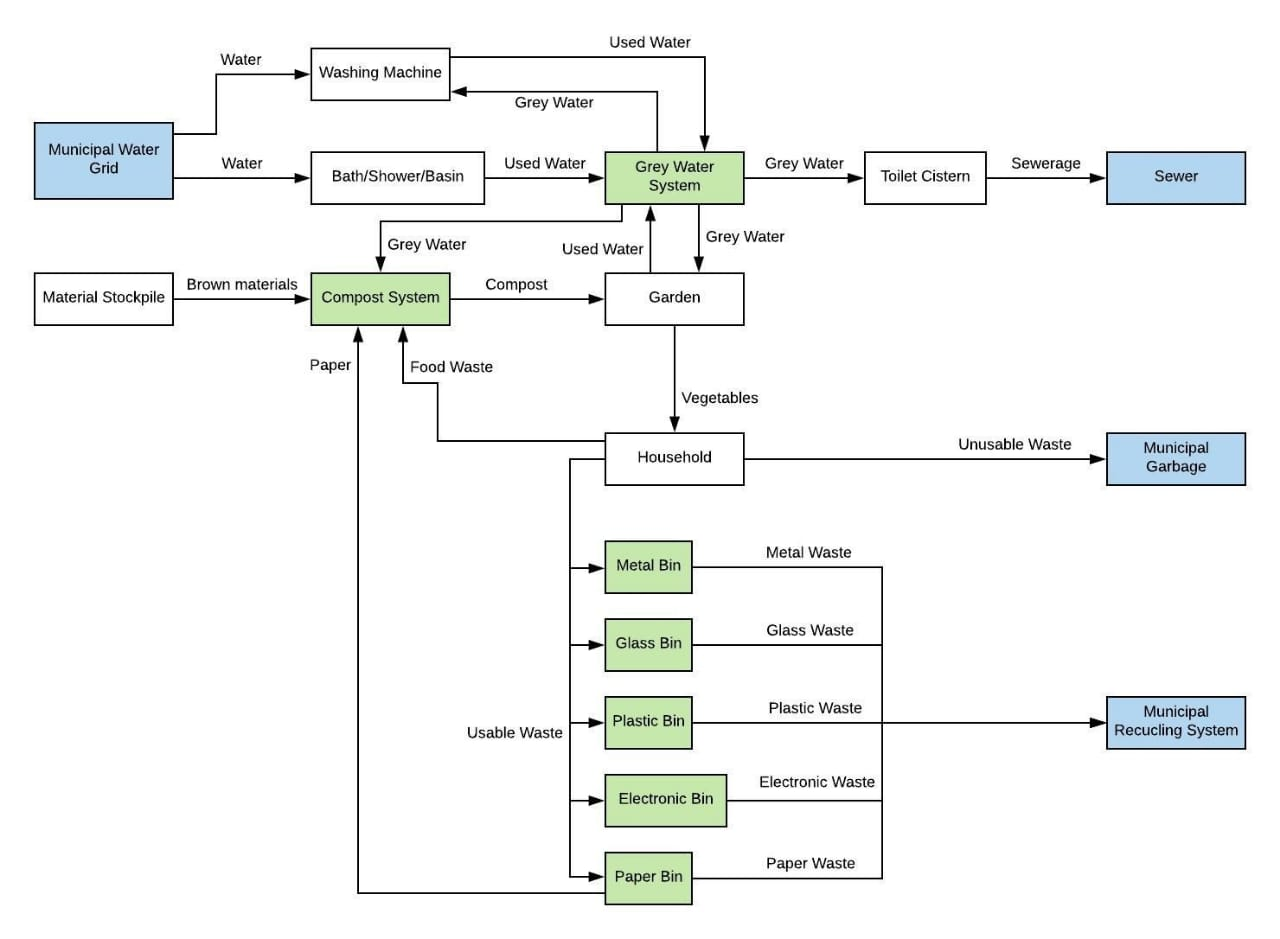
\includegraphics[scale = 0.34]{System_Diagram.jpg}
\caption{System Diagram}
\label{fig: systemDiagram}
\end{center}
\end{figure}


\section{Advanced Development Phase}

\subsection{Requirements Analysis}

\subsection{Functional Analysis and Design}

\subsection{Prototype Development}

\subsection{Development Testing}

\section{Engineering Procurement Phase}

\subsection{Requirements Analysis}

\subsection{Functional Analysis and Design}

\subsection{Component Design}

\subsection{Design Validation}

\section{Integration and Evaluation Phase}

\subsection{Test Planning and Preparation}

\subsection{System Integration}

\subsection{Developmental System Testing}

\subsection{Operational Test and Evaluation}

\chapter{Post Development Stage}

\section{Production and Deployment Phase}

\subsection{Transitions from Development to Production}

\subsection{Production Operations}

\section{Operations and Support Phase}
Installation and test (system integration site, internal and external, disruptive or non-disruptive installation, early system operational difficulties encountered or that could be encountered, operational personnel)
Logistics, Support and Maintenance schedule
System Upgrades (hard and software upgrade plans)

\chapter{Software Design and System Dynamics}
This phase is required to study the behaviour and structure of a system by carrying out sensitivity analysis tests. Only select critical elements or more as deemed fit from the designed system and apply to these to the modelling capability of a chosen software.
Your algorithm/software approach should be such that a change in the value of one element’s input can be quantitatively seen in other elements within the network. [Use software such as: Anylogic, Vensim, Stella, Dynamo++ etc]
Phase II is tied to your ability to demonstrate sensitivity analysis, structure and behaviour of a system resulting from a change in one or more parameters of some system elements.

\section{Core 9 System Design Structure}

\section{System Dynamics Analysis}
==35marks==

\section{Selected Elements for System Dynamics Analysis}
==10/35marks==
Reason for selecting these elements in a situation where the new network for SD differs from the main designed network ==5/35marks==

\section{Sensitivity Analysis}
==20/35marks==
Simulation runs to demonstrate sensitivity analysis, changed system behaviour etc 

\chapter{Conclusion}
\acresetall
This is the chapter where you add \emph{concluding} remarks. It is not a summary.

\bibliography{Example}

\appendix
\chapter{Some data as appendix}

\end{document}
